\documentclass[10pt, a4paper]{article}



\usepackage{lrec}
%\usepackage{multibib}
%\newcites{languageresource}{Language Resources}
\usepackage{graphicx}
\usepackage{tabularx}
\usepackage{soul}
% for eps graphics
\usepackage{subcaption}

\usepackage{amsmath}

\usepackage[T1]{fontenc}

\usepackage{epstopdf}
%\usepackage[latin1]{inputenc}
\usepackage[utf8]{inputenc} %% Render certain characters correct.
\usepackage{hyperref}
\usepackage{xstring}

\newcommand{\secref}[1]{\StrSubstitute{\getrefnumber{#1}}{.}{ }}

\title{Discriminating Between Similar Nordic Languages}

\name{René Haas, Leon Derczynski}

\address{IT University of Copenhagen \\
         \{renha, leod \}@itu.dk\\}


\abstract{Automatic language identification is a challenging problem and especially discriminating between closely related languages is one of the main bottlenecks of state-of-the-art language identification systems. This paper presents a machine learning approach for automatic language identification for the Nordic languages, which often suffer miscategorisation by existing state-of-the-art tools. Concretely we will focus on discrimination between the six Nordic languages: Danish, Swedish, Norwegian (Nynorsk), Norwegian (Bokmål), Faroese and Icelandic.
\\ 
\newline \Keywords{DSL, NLP, Language Identification, Machine Learning} }

\begin{document}

\maketitleabstract

\section{Introduction}
Automatic language identification is a challenging problem and especially discriminating between closely related languages is one of the main bottlenecks of state-of-the-art language identification systems.\cite{DSL2014}

This paper presents a machine learning approach for automatic language identification for the Nordic languages. Concretely we will focus on discrimination between the six Nordic languages: Danish, Swedish, Norwegian (Nynorsk), Norwegian (Bokmål), Faroese and Icelandic.

This papers explore different ways of extracting features from a corpus of raw text data consisting of Wikipedia summaries in respective languages and evaluates the performance of a selection of machine learning models.

Concretely we will compare the performance of classic machine learning models such as Logistic Regression, Naive Bayes, Support vector machine, and K nearest Neighbors with more contemporary neural network approaches such as Multilayer Perceptrons (MLP) and Convolutional Neural Networks (CNNs).

After evaluating these models on the Wikipedia data set we will continue to evaluate the best models on a data set from a different domain in order to investigate how well the models generalize when classifying sentences from a different domain.

\section{Related Work}

The problem has been investigated in recent work \cite{DSLEvaluation}\cite{DSL2015} which discuss the results from two editions of the ``Discriminating between Similar Languages (DSL) shared task". Over the two editions of the DSL shared task different teams competed to develop the best machine learning algorithms to discriminate between the languages in a corpus consisting of 20K sentences in each of the languages: Bosnian, Croatian, Serbian, Indonesian, Malaysian, Czech, Slovak, Brazil Portuguese, European Portuguese, Argentine Spanish, Peninsular Spanish, Bulgarian and Macedonian.\\

\section{Data acquisition}
The first step when constructing a language classifier is to gather a data set. For this purpose I wrote a small script using the Wikipedia API for Python.\footnote{\url{https://pypi.org/project/wikipedia/}}\\

With the script I was able to download the summaries for randomly chosen Wikipedia articles in each of the languages which are saved to as raw text to 6 {\tt .txt} files of about 10MB each.\\

After the initial cleaning, which i will describe in the next section, the data set contains just over 50K sentences in each of the language categories. I chose to select two data sets with exactly 10K and 50K sentences respectively from the raw data set. In this way the data sets we will work with are balanced, containing the same number of data points in each language category.\\

Throughout this report we split these data sets, reserving 80\% for the training set and 20\% for the test set we use when evaluating the models.

\subsection{Data cleaning}
In this section I will briefly describe how the data set is initially cleaned and how sentences are extracted from the raw data.

\paragraph{Extracting sentences:}

The first thing we want to do is to divide the text into sentences.
This is generally a non-trivial thing to do. My approach is to first split the raw string by line break.
This roughly divides the text into paragraphs with some noise which we filter out in the last step.\\

We then extract shorter sentences with the sentence tokenizer ({\tt sent\_tokenize}) function from the NLTK\cite{nltk} python package. This does a better job than just splitting by {\tt '.'} due to the fact that abbreviations, which can appear in a legitimate sentence, typically include a period symbol.

\paragraph{Cleaning characters}
The initial data set have a lot of characters that do not belong to the alphabets of the languages we work with. Often the Wikipedia pages for people or places contain the name in the original language. For example a summary might contain Chinese or Russian characters which are arguably irrelevant for the purpose of discriminating between the Nordic languages.\\

To make the feature extraction simpler, and to reduce the size of the vocabulary, I chose to make the raw data lowercase and strip all characters with are not part of the standard alphabet of the six languages.\\

In this way we only accept the following character set
\begin{verbatim}
'abcdefghijklmnopqrstuvwxyzáäåæéíðóöøúýþ '
\end{verbatim}
and replace everything else with white space before continuing to extract the features.
For example the raw sentence
\begin{verbatim}
'Hesbjerg er dannet ved sammenlægning
 af de 2 gårde Store Hesbjerg
 og Lille Hesbjerg i 1822.'
\end{verbatim}
will after this initial cleanup be reduced to
\begin{verbatim}
'hesbjerg er dannet ved sammenlægning
 af de gårde store hesbjerg
 og lille hesbjerg i ',
\end{verbatim}
We thus make the assumption that capital letters, numbers and characters outside this character set do not contribute much information relevant for language classification.

\section{Baselines}

\subsection{Baseline With langid.py}

As a baseline to compare the performance of the models in we compare with an out of the box language classification system. ``langid.py: An Off-the-shelf Language Identification Tool." \cite{langID} is such a tool.\\

Out of the box langid.py comes with with a pretrained model which covers 97 languages. The data for langid.py comes from from 5 different domains: government documents, software documentation, newswire, online encyclopedia and an internet crawl.\\

We evaluated how well langid.py performed on the Wikipedia dataset. Since langid.py returned the language id ``no" (Norwegian) on some of the data points we restrict langid.py to only be able to return either ``nn" (Nynorsk) or ``nb" (Bokmål) as predictions. It is a quite peculiar feature of the Norwegian language that there exist two different written languages but three different language codes.\\

\begin{figure}[h!]
  \centering
  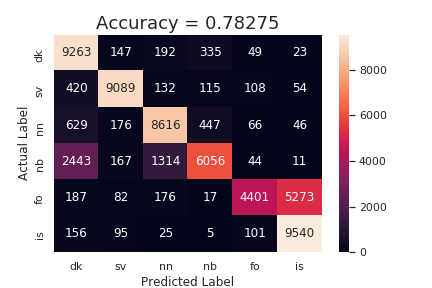
\includegraphics[width = 200pt]{figs/langid}
  \caption{Confusion matrix with results from langid.py on the full dataset with 300K data points. }
  \label{langid_confusion_matrix}
\end{figure}

In Figure~\ref{langid_confusion_matrix} we see the confusion matrix for the langid.py classifier. The largest errors are between Danish and Bokmål and between Faroese and Icelandic. We see that langid.py was actually able to correctly classify most of the Danish data points however approximately a quarter of the data points in Bokmål was incorrectly classified as Danish and just under and eighth was classified as Nynorsk.\\

Furthermore langid.py correctly classified most of the Icelandic data points however over half of the data points in Faroese was incorrectly classified as Icelandic.\\

\begin{table}
  \centering
  \begin{tabular}{ l | c | r }
    \hline
    Model               & Encoding  & Accuracy \\
    \hline
    Knn                 & cbow &  0.780\\
    Log-Reg             & cbow &  0.819\\
    Naive Bayes         & cbow &  0.660\\
    SVM                 & cbow &  0.843\\
    Knn                 & skipgram &  0.918\\
    Log-Reg             & skipgram &  \textbf{0.929}\\
    Naive Bayes         & skipgram &  0.840\\
    SVM                 & skipgram &  \textbf{0.928}\\
    Knn                 & char bi-gram  & 0.745\\
    Log-Reg             & char bi-gram  & 0.907\\
    Naive Bayes         & char bi-gram  & 0.653\\
    SVM                 & char bi-gram  & 0.905\\
    Knn                 & char uni-gram  & 0.620\\
    Log-Reg             & char uni-gram  & 0.755\\
    Naive Bayes         & char uni-gram  & 0.614\\
    SVM                 & char uni-gram  & 0.707\\
    \hline
  \end{tabular}
  \caption{Overview of results for the dataset with 10K data points in each language.}
  \label{baseline-results-10k}
\end{table}

\subsection{Baseline with linear models}

In the Table~\ref{baseline-results-10k} we see the results for running the models on a dataset with 10K data points in each language category. We see that the models tend to perform better if we use character bi-grams instead of single characters.\\

Also we see that logistic regression and support vector machines outperform Naive Bayes and K-nearest neighbors in all cases. Furthermore for all models we get the best performance if we use the skip-gram model from FastText.\\

Comparing the CBOW mode from FastText with character bi-grams we see that the CBOW model is on par with bi-grams for the KNN and Naive Bayes classifiers while bi-grams outperform  CBOW for Logistic Regression and support vector machines.\\


\section{Our Approach}

\subsection{Using FastText}

The methods described above are quite simple. We also compare the above method with FastText, which is a library for creating word embeddings developed by Facebook~\cite{BagOfTricks}. 

In the paper "Enriching Word Vectors with Subword Information" \cite{EnrichingWordVectors} the authors explain how FastText extracts feature vectors from raw text data. FastText makes word embedding using one of two model architectures: continuous bag of words (CBOW) or the continuous skip-gram model.

The skip-gram and CBOW models are first proposed in \cite{EfficientWordRepresentations} which is the paper introducing the word2vec model for word embeddings. FastText builds upon this work by proposing an extension to the skip-gram model which takes into account sub-word information.

Both models use a neural network to learn word embedding from using a context windows consisting of the words surrounding the current target word. The CBOW architecture predicts the current word based on the context, and the skip-gram predicts surrounding words given the current word.\cite{EfficientWordRepresentations}

\subsection{Using A Convolutional Neural Network}

While every layer in the MLP is densely connected such that each of the nodes in a layer is connected to all nodes in the next layer, in a convolution neural network we use one or more convolutional layers.

Convolutional Neural networks are very popular for image recognition but they can also be used for text classification \cite{textcnn_google}.

\begin{figure}[h!]
  \centering
  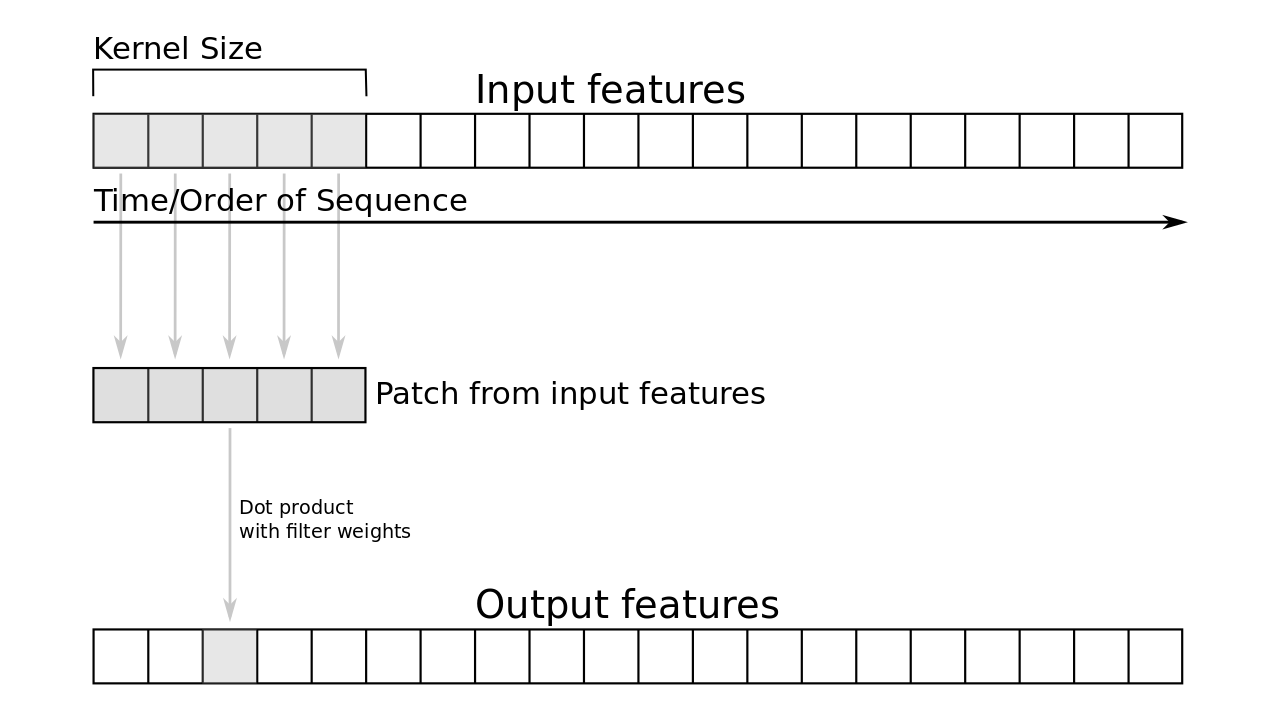
\includegraphics[width = 200pt]{figs/cnn_diagram}
  \caption{Diagram of Convolutional Neural network.}
  \label{cnn}
\end{figure}

The basic premise of a convolutional layer is illustrated in Figure~\ref{cnn}.\footnote{Source: \url{https://realpython.com/python-keras-text-classification/}} In a CNN you have a filter which slides over the input. The CNN then takes the dot product of the weights of the filter and the corresponding input features, before applying the activation function.

\section{Experiments}\label{sec:results}

In the following in Sec.~\ref{sec:data} we first describe the database, which we used to create different tensor models proposed in Sec.~\ref{sec:tensormodel}. 
Based on these, we present substructures which we found in the auxiliary latent space in Sec.~\ref{sec:subspace}. 
A qualitative comparison of the reconstruction quality of the two different versions of the tensor model is presented in  Sec.~\ref{sec:extmodel}. 
We proceed to quantitatively evaluate the effect of varying regularisation parameters on approximation and transfer in Sec.~\ref{sec:validation}, and then apply these findings by a qualitative results presented in Sec.~\ref{sec:approx}. 

\subsection{Facial Expression Database} \label{sec:data}
In this work, we use the Binghamton University 3D Facial Expression database (BU-3DFE)\cite{bu3dfe}. 
It contains 3D face scans and images of 100 persons (56 female and 44  male), with varying age (18-70 years) and diverse ethnic/races. 
Each subject was asked to perform the six basis emotions: anger, disgust, happiness, fear, sadness, and surprise, each with four levels of increasing expression strength. 
Additionally, for each participant the neutral face was recorded.
Hence, a total of 25 facial expressions is provided, recorded from two different rotations, %($\pm \pi/4$ from frontal)
i.e. left and right rotations, from which an additional morphed frontal image is provided.
% Maybe something this these?
% \input{tex/fig/Fig3/fig3.tex}

%\subsection{Subspace Analysis}
\subsection{Subspace Analysis of the Auxiliary Latent Space}
\label{sec:subspace}
% Sec.~\ref{sec:latent_space_embedding} describes how the face images of the BU3D-FE database can be embedded into the latent space of the StyleGAN1 and 2. The resulting latent vectors are then ordered into a data tensor, which is factorised by a HOSVD, as described in  Eq.~\ref{eq:matrix_hosvd}, leading to three different subspaces, represented by the matrices $\matr{U}_k$. 
The BU-3DFE database offers 7500 face images, see Sec.~\ref{sec:data}, %of 100 persons in 25 expressions, i.e. the 6 basic emotions in 4 intensity levels and neural, see Sec.~\ref{sec:data}.
which we embed into the latent space of StyleGAN1 and 2, as described in Sec.~\ref{sec:stylegan}, hence for each face image one latent vector is obtained. 
The resulting latent vectors are ordered into a 4way data tensor $T\in\R^{N\times P\times E \times R}$. %where $N$ is the number of elements of one latent vector, $P$ refers to 100 persons and $E$ are the 25 expressions. 
The 4-way data tensor is then factorised by the HOSVD, as described in \eqref{eq:matrix_hosvd} leading to four different subspaces %spanned by the columns of the associated orthogonal matrices
$\matr{U}_k$, $k=1,\ldots,4$. % reflecting the different dimensions of the data tensor. 
The first three dimensions of the expression subspace spanned by the columns of $\matr{U}_3$ are visualised in Fig.~\ref{fig:apathy_vs_neutral}\subref{subfig:subspaces}. 
It can be seen that the for each emotion, the four points of different varying expression strengths form linear trajectories, which intersect a new expression, which does not equal the neutral expression, nor the mean face. 
These three expressions were synthesised for the mean person and are illustrated in Fig.~\ref{fig:apathy_vs_neutral}. 
It can be seen that the mouth in the mean and the neutral expression is open and looks rather happy, whereas the mouth is closed in the newly synthesised  expression, hence we labelled it as \emph{apathetic} as in \cite{apathy,grasshof2020}. 
This confirms the findings from \cite{apathy,grasshof2020} based on the same database and others. 
Similarly, we utilise the structure found in the subspace by employing reasonable constraints for the optimisation procedure and hence improve the results for for new inputs, which we show in Sec.~\ref{sec:approx}. 

%based on data of 3D faces from the same database and an additional 2D database.
% To visualise the differences between the three expressions, each of them was synthesised and is illustrated in Fig.~\ref{fig:apathy_vs_neutral} on the mean person. It can be seen that the mouth in the mean and the neutral expression is open and looks rather happy, whereas the mouth is closed in the apathetic expression. 
%This shows that there is a structure in the subspaces, which we enforce to stick to by constrained optimisation described in Sec.~\ref{sec:optimisation} for new inputs. 
%  labelled as \emph{apathetic}. 
%%%%%
%It can be seen that the four points describing different expression strengths for each emotion (visualised in different colors) form trajectories and that these intersect in a new expression, which does not equal the neutral expression, nor the mean face, labelled as \emph{apathetic}. 
% % % FIGURE 5
\input{fig/Fig5/fig5.tex}


%\subsection{Vectorised vs. Extended Model}
\subsection{Vectorised vs. Stacked Style-Separated Model Model}
\label{sec:extmodel}

On the basis of the auxiliary latent space, we proposed to build two different versions of tensor models in Sec.~\ref{sec:tensormodel}. Both are based on a factorisation of different data tensors: 

(1) The \emph{vectorised model} which vectorises each latent code of one image and then orders them into a data tensor $T\in\R^{N\times P\times E\times R}$, and 

(2) the \emph{stacked style-separated model} $T_\text{style}\in\R^{S\times L\times P\times E\times R}$ which considers the $S=18$ styles of StyleGAN separately, and hence is based on $S$ style-specific tensors $T_s\in\R^{L\times P\times E\times R}$, $s=1,\ldots, S$, see Sec.~\ref{sec:extended_model}. 

In this section we compare the results obtained by the two models, each using the ALS procedure \eqref{eq:als} for optimisation. 
%we proposed to either build one tensor model $T$ $T^{(i)}$
%different models were proposed. 
%Fig.~\ref{fig:vec_vs_extended_model}
The results are illustrated in Fig.~\ref{fig:fig7}. It can be seen that the input images shown in Fig.~\ref{fig:fig7}\subref{subfig:reference}, are visually matched better by the \emph{stacked style-separated model}, presented in Fig.~\ref{fig:fig7}\subref{subfig:extended}, as compared to the results of the \emph{vectorised model} shown in Fig.~\ref{fig:fig7}\subref{subfig:vectorised}. This observation holds for test data samples of BU-3DFE shown in the top row, as well as for arbitrary examples shown in 2nd and 3rd row. 
Therefore, we conclude that the proposed adaptation considering the separate styles, improves the performance. 

\input{fig/Fig7/fig7.tex}

%%%%%%%%%%%%%%%%%%%%%%%%%%%%%%%%%%
\subsection{Validation of Regularisation Parameters}
\label{sec:validation}

The optimisation problem defined in \eqref{eq:lagrangian} contains two hyper parameters: $\lambda_1$ and  $\lambda_2$, which must be manually set.
%\eqref{eq:optimisation_problem} 
%The proposed optimisation procedures contain hyper parameters, which need to be manually set. 
In this section we investigate how they influence the quality of the results using the previously defined \emph{vectorised model} on the basis of the standardised latent codes, i.e. $T\in\R^{N\times P\times E\times R}$ in \eqref{eq:matrix_model}. 
%, based on the \eqref{eq:lagrangian}. 

First, we separate the data tensor into  training, validation and test set by a randomised 90/5/5 over the $P=100$ person identities. As a result, the validation set has a total of $5E R=5\cdot25\cdot3=375$ samples. 
We build one tensor model based on the training set. 

%intro
Then for each sample of the validation set $\vec{y}_i\in\mathcal{W}$ we estimate the parameter tensor $\widehat{Q}_i$ by ALS in \eqref{eq:als}, which estimates the  parameter tensor  $\widehat{Q} = \widehat{\vec{q}}_\text{person} \otimes \widehat{\vec{q}}_\text{expression} \otimes \widehat{\vec{q}}_\text{rotation}$. The input sample is then approximated by $\widehat{\vec{y}}_i = \tau(\widehat{Q}_i)$ as in \eqref{eq:taugam}. 
%reconstruction
We define the approximation error between true $\vec{y}$ and estimated auxiliary latent code $\widehat{\vec{y}}_i$ as $\epsilon_\text{approx} =\epsilon(\widehat{\vec{y}},\vec{y})$ where the error metric is defined as
$\epsilon(\widehat{\vec{y}},\vec{y}) \equiv  \norm{\widehat{\vec{y}}-\vec{y}}^2$. 
%expression transfer
Additionally, we evaluate the transfer errors resulting from exchanging estimated parameters $\hat{\vec{q}}_k$ by known values $\tilde{\vec{q}}_k$. Hence using $\widetilde{\vec{y}}_\text{expr} \equiv \tau(\widehat{\vec{q}}_{\text{person}} \otimes \widetilde{\vec{q}}_{\text{expr}}\otimes \widehat{\vec{q}}_{\text{rot}})$ give rise to an expression transfer error which we define as $\epsilon_\text{expr}\equiv\epsilon(\widetilde{\vec{y}}_\text{expr},\vec{y})$. 
%rotation transfer
Analogously, we define a rotation transfer error $\epsilon_\text{rot} \equiv \epsilon(\widetilde{\vec{y}}_\text{rot},\vec{y})$ by calculating error arising from only changing the rotation part of the parameter tensor: $\widetilde{\vec{y}}_\text{rot} \equiv \tau(\widehat{\vec{q}}_{\text{person}}\otimes\widehat{\vec{q}}_{\text{expr}}\otimes\widetilde{\vec{q}}_{\text{rot}})$.

The three error metrics $\epsilon_\text{approx}$ $\epsilon_\text{expr}$, and $\epsilon_\text{rot}$ are calculated, for each sample, with varying hyper parameter values $\lambda_1$ and $\lambda_2$. Then the mean over all the sample-wise errors is computed, leading to $\overline{\epsilon}_{\cdot}$. 
The results are illustrated in Fig.~\ref{fig:hyper_param_errors}, where from top to bottom the mean errors are presented for: approximation error, expression transfer, and rotation transfer. 
In general it can be seen that the approximation error does not fluctuate as much as the other two error metrics. 
Fig.~\ref{fig:hyper_param_errors}\subref{subfig:l1penalty} indicates that high values of $\lambda_1$ should be chosen for rotation transfer, while for expression transfer $\lambda_1\approx 1$ seems to be a reasonable choice. 
Fig.~\ref{fig:hyper_param_errors}\subref{subfig:l2penalty} reveals that for $\lambda_2 \approx 1$ all error metrics are small, and hence this interval is a good choice for multiple usages. 
In the following section we use these findings by selecting specific parameter weights, and then perform expression and rotation transfer on samples the test set. 
\input{fig/Fig8/fig8_overlay.tex}
\subsection{Regularisation and Parameter Transfer}
\label{sec:approx}
In the previous section Sec.~\ref{sec:validation} quantitative results on expression and rotation transfer were presented, with respect to varying hyper parameters. 
%Here we pr
% In this section we show that the tensor model proposed in Sec.~\ref{sec:tensormodel} can be used to approximate unseen samples by employing the optimisation procedures described in Sec.~\ref{sec:optimisation}. 
In this section we estimate the parameters $\widehat{Q}$ for an unknown image $\vec{x}$ of the test set. We can retrieve an image from the estimated parameters by applying the composed transformation $\vec{x}\approx\widehat{\vec{x}}= g(\tau(\widehat{Q}))$. 
Additionally, we perform expression and rotation transfer by replacing one of the three estimated parameter vectors by known values, as described before. 
We do this for the regularised model, i.e. $\lambda_1>0,~\lambda_2>0$, and the non-regularised model, by choosing $\lambda_1=\lambda_2=0$. 
In Fig.~\ref{fig:fig9} the top row shows how well the ground truth (GT) presented in Fig.~\ref{fig:fig9}(a) can be approximated by Fig.~\ref{fig:fig9}(b) the non-regularised solution and Fig.~\ref{fig:fig9}(c) the regularised solution. When comparing them it seems that the non-regularised solution matches the GT slightly better. 
This statement also holds for the expression transfer shown in Fig.~\ref{fig:fig9}(b). 
However comparing the rotation transfer Fig.~\ref{fig:fig9}(c) shows that the regularised solution (bottom row) clearly outperforms the non-regularised solution (top row). Because in the non-regularised solution the resulting image is not recognisable as a face anymore at all, while the regularised solution is not deformed and the rotation of the depicted faces conform to the GT.
\input{fig/Fig9/fig9.tex}


% \begin{align}
%\frac{1}{N}\norm{\vec{y}-\vec{y}}^2   
% \epsilon_\text{approx} &=\epsilon(\widehat{\vec{y}},\vec{y}),\\
% \intertext{where the error metric is defined as}
% \epsilon(\widehat{\vec{y}},\vec{y}) &\equiv  \norm{\widehat{\vec{y}}-\vec{y}}^2. %\equiv \tensor{R}{_{\mu}} \tensor{R}{^{\mu}} 
%\intertext{is the error metric.}
%\vec{\vec{y}}&= f(\widehat{\vec{q}}_\text{person},\widehat{\vec{q}}_\text{expression},\widehat{\vec{q}}_\text{rotation})\\
% \end{align}
%is the approximated face image. 
%$\frac{1}{N}\norm{\vec{y}-\vec{y}}^2$ 
%$\hat{\vec{q}}_i \to \tilde{\vec{q}}_i$, i.e. for 
% \begin{align}
% \epsilon_\text{expr}&\equiv\epsilon(\widetilde{\vec{y}}_\text{expr},\vec{y}),\\
% %\widetilde{\vec{y}}_\text{expr} &\equiv \tau(\widehat{\vec{q}}_{\text{person}},\widetilde{\vec{q}}_{\text{expr}},\widehat{\vec{q}}_{\text{rot}}), \\
% \intertext{and with $\widetilde{\vec{y}}_\text{rot} \equiv \tau(\widehat{\vec{q}}_{\text{person}},\widehat{\vec{q}}_{\text{expr}},\widetilde{\vec{q}}_{\text{rot}})$ the rotation transfer error as}
% \epsilon_\text{rot}&\equiv\epsilon(\widetilde{\vec{y}}_\text{rot},\vec{y}).%\\
% %\widetilde{\vec{y}}_\text{rot} &\equiv \tau(\widehat{\vec{q}}_{\text{person}},\widehat{\vec{q}}_{\text{expr}},\widetilde{\vec{q}}_{\text{rot}}).
% \end{align}

%%%%%%%%%%%%%%%%%%%%%%%%%%%%%%%



%we present qualitative results on the basis of the test set.
%, such that for each hyper parameter value exactly one value for each error metric remains, which can then be represented by lines. 
% In Fig.~\ref{fig:hyper_param_errors}\subref{subfig:l1penalty} the $x$-axis refers to the hyper parameter $\lambda_1$, which weights the L1 penalty, while in Fig.~\ref{fig:hyper_param_errors}\subref{subfig:l2penalty} the $x$-axis refers to $\lambda_2$, which weights the L2 penalty. 

%
% \begin{align}
% P_\text{expr,transfer} = (\widehat{\vec{q}}_{\text{person}}\otimes\widetilde{\vec{q}}_{\text{expr}}\otimes\widehat{\vec{q}}_{\text{rot}})
% \end{align}
% \begin{align}
%     \widetilde{Y}_\text{e} = S(\widehat{\vec{q}}_{\text{person}}\otimes\widetilde{\vec{q}}_{\text{expr}}\otimes\widehat{\vec{q}}_{\text{rot}})
% \end{align}
%


\section{Analysis}

\subsection{Principal Component analysis and t-SNE}
To gain additional insight on how the different word embedding capture important information about each of the language classes we thought it would be interesting to try and visualize the embeddings using two different techniques for dimensionality reduction.

No matter which way we choose to extract the feature vectors they belong to a high dimensional feature space and in order to do visualization we need to project the feature vectors down to 2d space.

To do this we have implemented two different methods: Principal Component Analysis (PCA) which we will compare with T-distributed Stochastic Neighbor Embedding (t-SNE).
Here we will begin with a brief explanation of the two techniques and proceed with an analysis of the results.

\paragraph{Principal Component Analysis}

The first step is to calculate the covariance matrix of the data set.
The components of the covariance matrix is given by

\begin{align}
K_{X_i,X_j} = E[(X_i - \mu_i )(X_j -  \mu_j)]
\end{align}

where $X_{i}$ is the $i$th component of the feature vector and $\mu_{i}$ is the mean of that component.

In matrix form we can thus write the covariance matrix as
\begin{align}
K(\mathbf{x},\mathbf{z}) =
\begin{bmatrix}
    \text{cov}(x_1,z_1) &  \dots  & \text{cov}(x_1,z_n) \\
    \vdots & \ddots     & \vdots \\
    \text{cov}(x_n,z_1) & \dots  & \text{cov}(x_n,z_n) \\
\end{bmatrix}
\end{align}
The next step is to calculate the eigenvectors and eigenvalues of the covariance matrix by solving the eigenvalue equation.
\begin{align}
\det (K v-\lambda v) = 0
\end{align}
The eigenvalues are the variances along the direction of the eigenvectors or "Principal Components". To project our data set onto 2D space we select the two eigenvectors largest associated eigenvalue and project our data set onto this subspace.

In Figure \ref{pca} we see the result of running the PCA algorithm on the wikipedia data set where we have used character level bigrams as features as well as the cbow and skipgram models from FastTest.


\begin{figure}[h!]
    \centering
    \begin{subfigure}[b]{0.47\textwidth}
        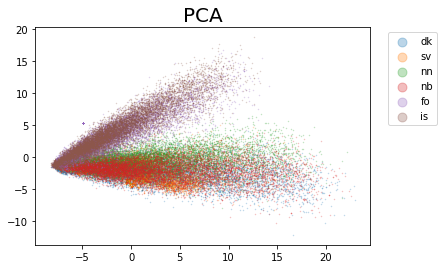
\includegraphics[width=\textwidth]{figs/pcachar2}
        \caption{Character bigram}
    \end{subfigure}
    ~
    \begin{subfigure}[b]{0.47\textwidth}
        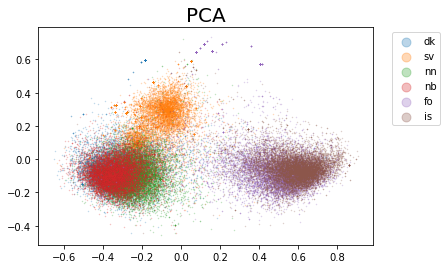
\includegraphics[width=\textwidth]{figs/pcacbow1}
        \caption{Fasttext cbow}
    \end{subfigure}
    ~
    \begin{subfigure}[b]{0.47\textwidth}
        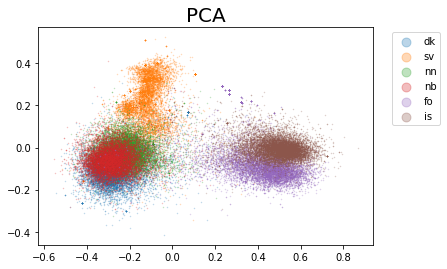
\includegraphics[width=\textwidth]{figs/pcaskipgram1}
        \caption{Fasttext skipgram}
    \end{subfigure}
    \caption{Dimensionality reduction using PCA}
    \label{pca}
\end{figure}

In the figure for encoding with character level bi-grams the PCA algorithm resulted in two elongated clusters. Without giving any prior information about the language of each sentences the PCA is apparently able to discriminate between Danish, Swedish, Nynorsk and Bokmål on one side and Faroese and Icelandic on the other since the majority of the sentences in each language belong to either of these two clusters. With the FastText implementations we observe three clusters.s

For both cbow and skipgram we see a distinct cluster of Sweedish sentences. When comparing the two FastText models we see that the t-SNE algorithm with skipgrams seems to be able to separate the Faroese and Icelandic data points to a high d ecree compared with the cbow model. Also for the cluster identified with the sentences with Danish, Bokmål and Nynorsk the skipgram models seem seem to give a better separation, however to a lesser degree than with the two former languages.

\paragraph{t-SNE}

The T-distributed Stochastic Neighbor Embedding method was first proposed in 2008 in the paper "Visualizing Data using t-SNE"\cite{tsne}.

In the paper the authors explain the theory behind the algorithm which we  will make a brief summary of here.

Suppose you pick a data point $x_i$, then the probability of picking another data point $x_j$ as a neighbor to $x_i$ is given by
\begin{align}
p_{ji}= \frac{\exp (|| x_i - x_j ||^2/2\sigma_i^2 )}{\sum_{k\neq i} \exp (|| x_i - x_k ||^2/2\sigma_i^2 )}
\end{align}

Now having this probability distribution the goal is to find the low-dimensional mapping of the data points $x_i$ which we denote $y_i$ follow a similar distribution. To solve what is referred to as the "crowding problem" the t-SNE algorithm uses the Student t-distribution which is given by
\begin{align}
q_{ij}= \frac{ (1+|| y_i - y_j ||^2 )^{-1}}{\sum_{k\neq l} (1+|| y_k - y_l ||^2 )^{-1}}
\end{align}
Now finally for optimizing this distribution is done by using gradient decent on the Kullback-Leibler divergence which is given by
\begin{align}
\frac{\delta C}{\delta y_i}= 4 \sum_j (p_{ij} - q_{ij})(y_i-y_j)(1+ || y_i - y_j ||^2  )^{-1}
\end{align}
The result from running the t-SNE algorithm on the Wikipedia data set can be seen in Figure \ref{tsne}. As was the case with the PCA algorithm it appears that the encoding with FastText seem to capture the most relevant information to discriminate between the languages, especially the skip-gram mode seems to do a good job in capturing relevant information.

\begin{figure}[h!]
    \centering
    \begin{subfigure}[b]{0.47\textwidth}
        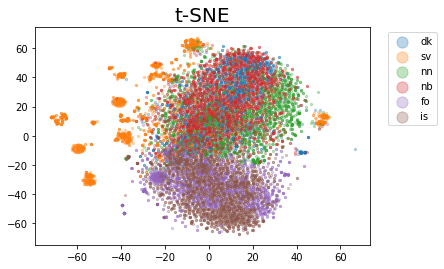
\includegraphics[width=\textwidth]{figs/tsnechar2}
        \caption{Character bi-gram}
    \end{subfigure}
    ~
    \begin{subfigure}[b]{0.47\textwidth}
        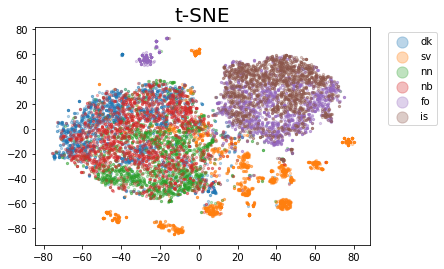
\includegraphics[width=\textwidth]{figs/tsnecbow1}
        \caption{FastText CBOW}
    \end{subfigure}
    ~
    \begin{subfigure}[b]{0.47\textwidth}
        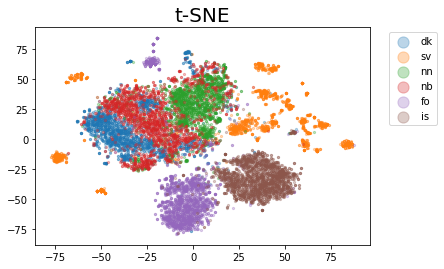
\includegraphics[width=\textwidth]{figs/tsneskipgram1}
        \caption{FastText skip-gram}
    \end{subfigure}
    \caption{Dimensionality reduction using t-SNE}
    \label{tsne}
\end{figure}


Here we recover some interesting information about the similarity of the languages. The data points in Bokmål lies in between those in Danish and Nynorsk while Icelandic and Faroese have their own two clusters which are separated from the three former languages. 

This is in good agreement with what we already know about the languages. Interestingly the Swedish data points and quite scattered and the t-SNE is not able to make a coherent Swedish cluster.

This does not however mean that the Swedish datapoint are not close in the original space. Some care is needed when interpreting the plot since t-SNE groups together data points such that neighboring points in the input space will tend to be neighbors in the low dimensional space.

If points are separated in input space, t-SNE would like to separate them in the low dimensional space however it does not care how far they are separated. So clusters that are far away in the low dimensional space are not necessarily far away in the input space.

\subsection{Discussion}
We used the dimensionality reduction techniques PCA and t-SNE to make visualizations of feature vectors obtained by making a one-hot encoding with character bi-grams and with the two modes from FastText.

These unsupervised techniques was able to separate the sentences from Wikipedia into different clusters.
Without any prior knowledge about the actual language of each sentence these techniques indicated that the six languages can be divided into three main language categories: (1) Danish Nynorsk Bokmål (2) Faroese Icelandic and (3) Swedish.


Generally the supervised models had the largest errors when discriminating between languages belonging to either of the language groups mentioned above.

For the "classical" models we saw that Logistic Regression and support vector machines achieved better performance than Knn and Naive Bayes, where the latter performed the worst. This was true in all cases irrespective of the method of feature extraction.

Additionally we saw that when we used feature vectors from the FastText skip-gram model the classification models achieved better results than when using either FastText CBOW or character n-grams.

Generally we saw that increasing the number of data points lead to better performance. When comparing the CNN with the "classical" models however the CNN performed better than any of the other models even when trained on less data points. In this way it seems that the CNN is able to learn more from less data when compared to the other models.

\section{Conclusions}
\label{sec:conclusion}

%+ tensor model in auxiliary latent space
%+ embedding of BU3DFE ()<maybe mention the compotational cost and resnet to decrease that embedding speed approx  (7500 data points) (2000 epochs)  (8 it/s ) =520hrs /21 days on tesla P100 (colab)

%+ previous findings confirmed: apathy mode 
%+ semantic subspaces
%- ?gradient descent and 
% Einstein Notation? could be its own point since we change the formalism non trivially when we introduce the combined rank 1 parameter tensor
%+ applications: approximation, expression and rotation transfer.

%Summary 
In this work, we have proposed $\tau$GAN a tensor based model for the auxiliary latent space of the StyleGAN. 
We first embedded the face database BU3DFE into the latent space. The resulting latent codes were stored into a multi dimensional  array or the data tensor, whose factorisation by HOSVD then yields semantically meaningful subspaces. We demonstrate the applicability approach by producing intuitive parametrisation for semantic face editing. 
%
%subspace (apathy)
Specifically, we were able to generalise the earlier result \cite{apathy} from feature-based face analysis:  %that suggested an alternative origin for the expressions
the expression subspace of the latent space namely has the structure where the expression trajectories meet in 
a specific emotionless face, the \emph{apathetic} expression, which is different from the mean or neutral face and the face. 
%
We evaluated our approach by quantitatively and qualitatively, and compared different versions of the proposed tensor models on the basis of approximation of unseen samples, and demonstrated stability in transfer of expression and rotation. From the results, we conclude that the proposed approach is powerful way for characterising and parameterising the latent spaces of StyleGAN.
%
%%%%%%%% Future work: keep it super short
In future, we intend to release a database by drawing samples from our auxiliary latent space. 

%\paragraph{Summary}

%\paragraph{Future work}

% \paragraph{Bigger and Better ResNet}
% Embedding a full data set of the scale of BU3D-FE into latent space is a very computationally intensive task. The estimated embedding time with 8it/s and for configuration B is 390 GPU hours on a single Tesla P100. The training of a larger (and hopefully better) ResNet would speed up the process by estimating better initial conditions for the VVG optimization. This would lower "the barrier of entry" for embedding data sets into the StyleGAN latent space.

% \paragraph{Time series data}
% Now, assuming we are able to estimate model parameters for an arbitrary reference image. The next logical step would be to estimate parameters for a time series and see how the parameters evolve. Each face in the tensor model is essentially a linear combination of the subspace basis vectors. We could model the time dependency of the expansion coefficients with Fourier analysis.

% \paragraph{Masking as post processing}
% In the configuration $\alpha$ run of the BU3D-FE latent space embedding we used the masking option from the code by \cite{pbaylies}. Having the unmasked latent vectors, it should be possible to add the mask as a post embedding step. This could be a way to augment the data. 

% \paragraph{Missing data}
% It is possible to define a generalized HOSVD which allows for missing data. This has been investigated in \cite{face2005}. It would be very interesting to implement a generalized model which allows for missing data, as this would make it possible to construct a tensor model on a less structured data set than the BU3D-FE database.  

% \paragraph{Creation of a synthetic data set based on the tensor model}
% We cannot release the tensor model since it is an approximation to the BU3D-FE data set which is under  Copyright by the authors. Our model can however generate synthetic faces with known parameters which do not exist in the BU3D-FE database. In principle we could generate a new synthetic data set, centered around the StyleGAN null\footnote{Mean face of StyleGAN, which ever version.} face, and then construct another tensor model on the synthetic data. 

% % \paragraph{Direct model embedding}
% % Another idea is to extimate the  model parameters directly from image use the VGG approach  to embed directly into our mode.skip the latent code. 


% \paragraph{Variational Auto encoders}
% GANs are not the only promising candidate for an neural network architecture for photo realistic image synthesis. It has been shown that "Vector Quantized" \cite{vqvae} \cite{vqvae2} Variational auto encoder are also able to synthesize high quality images of faces. It would be interesting to test the tensor model approach the latent space of these novel Variational Autoencoders.
 


% \begin{itemize}
%     \item We only consider using the same regularisation parameters along all modes. Maybe results would improve by allowing regularization parameters for each mode
% \item Better grip on regularization parameters: Allow for separate numerical  values for each mode.\footnote{And in case of the extended model- each style. }
% \item Time dependency: We can model the time dependency of model parameters by analyzing video.
% \item The VGG shortcut: We should be able to skip the intermediate embedding into $\mathcal{W}$ space by approximating model parameters directly using the VGG approach 
% \item ResNet: We can train an even larger ResNet for StyleGAN2
% \item Try this model on the StyleGAN $\mathcal{Z}$ space.
% \end{itemize}



\section{References}
\label{main:ref}

\bibliographystyle{lrec}
\bibliography{references}


\end{document}
